% !TeX root = ../main.tex

\chapter{數值模型結果}

\section{智利參考模型}
\subsection{初始模型設定}\label{智利參考模型初始模型設定}
本研究建立一個長1200公里、深300公里的長方形二維剖面,包含一段長425公里的海洋岩石圈與775公里的大陸板塊,在兩個板塊交界處,建立一段長度31公里傾角35度的隱沒板塊,交接處區域的溫度較高,方便隱沒帶發育。
智利參考模型設計見圖\ref{fig::reference Nazca model}。
海洋岩石圈年齡為40個百萬年(\citealp{muller2019}),包含1.5公里厚的沉積物、6公里厚的玄武岩與2.5公里厚的綠泥岩,其熱構造由\ref{熱邊界條件}節式\ref{eq:Half Space Model}提及的半空間冷卻模型決定。

\begin{figure*}[hb]
    \centering
    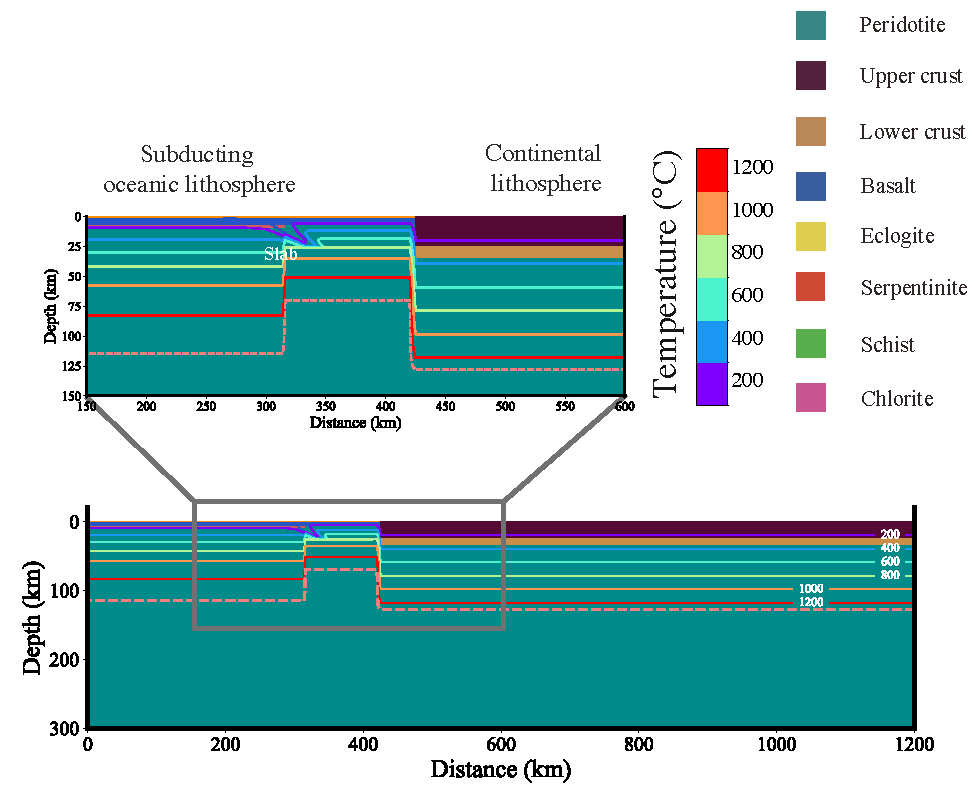
\includegraphics[width=6in]{Ref_Nazca.pdf}
    \caption[智利參考模型設計與邊界條件示意圖]{智利參考模型設計與邊界條件示意圖}
    \label{fig::reference Nazca model}
\end{figure*}

大陸岩石圈包含25公里厚的上部地殼(upper crust)與10公里厚的下部地殼(lower crust),由於秘魯與智利平坦隱沒區域的大陸地溫梯度資料較少,過去研究對該地區熱構造並沒有很好的約束,僅透過重力資料推測彈性岩石圈厚度大約130-140公里(\citealp{perez2008}),因此模型設定地溫梯度以每公里攝氏10.15$^{\circ}$線性遞增至130公里深設為岩石圈底部1330$^{\circ}$。
模型中地表溫度皆為攝氏10$^{\circ}$,模型底部溫度固定攝氏1330$^{\circ}$。

由於現生地震學觀測研究提及該地區地震活動度大,且地函岩石圈速度較高、板塊脫水作用不活躍(見\ref{秘魯與智利隱沒帶地球物理觀測}節),因此智利參考模型的蛇紋岩化橄欖岩厚度參數設定為5公里。模型左邊界從地表至300公里深皆以等速率每年6公分往右移動,右邊界則固定不動。
本研究速度參考來自於\citealp{o2005uncertainties},使用印度-大西洋熱點參考座標(Indo-Atlantic hotspot reference frame)中的相對板塊運動模型計算(\citealp{schellart2008global})。
模型上邊界為自由表面,而下邊界則為開放邊界,物質可自由進出。

需要注意現今的秘魯與智利平坦隱沒區皆落在安地斯山脈造山範圍,然而本參考模型沒有包含造山運動。
就現今觀測資料來看,平坦隱沒事件早於安地斯造山事件(\citealp{chen2019southward}; \citealp{hu2021southward}),兩者並沒有直接關係。


\subsection{智利參考模型結果}\label{智利參考模型結果}
智利參考模型產生一深度約100-110公里、長度約300公里的平坦段。
圖\ref{fig::Nazca_Ref_26}至圖\ref{fig::Nazca_Ref_150}為智利參考模型每5個百萬年之結果。

在隱沒初始時期,隱沒作用產生的速度場促使地函流上湧,導致地函楔溫度升高,同時強烈的岩石變形與破壞導致隱沒板塊交界處產生摩擦熱,海洋地殼溫度被動上升。
岩石在一系列的加溫下發生相變,隱沒地殼上的玄武岩相在深度40-50公里處左右相變成緻密的榴輝岩相,如圖\ref{fig::Nazca_Ref_26}a所示。
榴輝岩相密度遠大於周遭地函密度,顯著的密度差造成隱沒系統中的重力不穩定,促使隱沒板塊驅動力產生,隱沒系統得以順利發育,隱沒帶密度剖面見圖\ref{fig::Nazca_Ref_26}c。

海洋地殼上的沉積物在隱沒過程中絕大比例在海溝處堆積,形成厚度約10公里的增積岩體,僅有少部分沉積物被帶入地函中,這些沉積物與海水隨著地殼進入高溫高壓環境。
離開近地表後,地殼上的黏土礦物逐漸進入不穩定狀態,釋放出晶格中的水分,導致地函楔中的橄欖岩發生水合作用(hydration reaction)而相變成蛇紋岩化橄欖岩(serpentinized peridotite),其與隱沒的沉積物一同在地函楔中形成強度低的低黏滯度通道(low viscosity channel),見圖\ref{fig::Nazca_Ref_26}b與圖\ref{fig::Nazca_Ref_51}b模型黏滯度剖面。

在地函較深處,蛇紋岩化橄欖岩進入更高溫的環境發生脫水,於攝氏700$^{\circ}$處相變回橄欖岩。
由於攝氏700$^{\circ}$的環境下岩石幾乎都以黏性變形為主,因此低黏滯度通道在蛇紋岩化橄欖岩脫水後依然存在於板塊交界處中。

海洋板塊中的綠泥石橄欖岩在120-130公里深處發生脫水,相變成普通的橄欖岩。
儘管綠泥石橄欖岩脫水作用導致地函楔中的熔點下降,然而隱沒早期板塊溫度較低,即便進入地函楔中依然難以達到岩石熔點。

隱沒早期強烈的聚合作用在大陸岩石圈攝氏600$^{\circ}$等溫線之上方產生一厚度25公里、寬度150公里的高壓帶,詳見圖\ref{fig::Nazca_Ref_26}d動態壓力剖面紅色區域。
該高壓帶在10 Myr便消失,隨著隱沒持續進行,低黏滯度通道的存在隔絕上覆板塊、隱沒板塊與地函楔之間的物質交換,地函楔黏滯度高,地函流流動度受限。
在10 Myr,地函楔頂部、板塊交界處壓力降低,於80-120公里深處形成低壓區,見圖\ref{fig::Nazca_Ref_51}d深藍色區域。 
低壓區域促使動水壓力增加,為隱沒板塊施予一由隱沒板塊下地函(subslab mantle)指向地函楔的壓力梯度力,直接促使隱沒板塊傾角(dip)快速降低(見圖\ref{fig::Nazca_Ref_time})。

隨著隱沒板塊傾角降低,其下方因承受強烈彎曲(bending),在模型時間10-15 Myr之間於地函楔低壓區下方、隱沒地函岩石圈(subducting mantle lithosphere)處形成另一寬度約100公里的高壓區,見圖\ref{fig::Nazca_Ref_76}d紅色區域。
隱沒板塊下方的高壓帶與隱沒板塊上方的低壓帶平行於隱沒板塊,在隱沒板塊上
產生壓力梯度力,該力垂直作用於隱沒板塊。
在轉動系統中,壓力梯度力造成該隱沒段於逆時針方向上的力矩急遽增大,見圖\ref{fig::Nazca_Ref_time},因此在模型時間15 Myr後形成平坦隱沒。

這段時間內因隱沒傾角漸緩,地函楔橄欖岩在壓力不變的情形下溫度逐漸上升,有部分岩石通過固相線,發生些許部分熔融事件,部分熔融位置於圖\ref{fig::Nazca_Ref_76}c中黃點處,部分熔融比例見圖\ref{fig::Nazca_Ref_melting_time}a。

隨後模型至30 Myr,平坦隱沒持續發育,其深度大致與原先大陸岩石圈攝氏800$^{\circ}$等溫線深度相同,在模型中約略100-120公里深(圖\ref{fig::Nazca_Ref_76}a、\ref{fig::Nazca_Ref_101}a、\ref{fig::Nazca_Ref_126}a、\ref{fig::Nazca_Ref_150}a)。

因低黏滯度通道狹窄,隔絕地函流進入地函楔中,因此隱沒板塊上方的黏滯度持續維持低壓狀態。
此外,平坦隱沒上凹區域因強烈彎曲形成高壓帶,與板塊上方地函低壓帶形成的壓力梯度同樣垂直於隱沒板塊,因此在20 Myr之後,與重力力矩相比,動水壓力力矩維持穩定優勢,隱沒板塊與上覆板塊被牢牢吸住(圖\ref{fig::Nazca_Ref_76}b, d、\ref{fig::Nazca_Ref_101}b, d、\ref{fig::Nazca_Ref_126}b, d、\ref{fig::Nazca_Ref_150}b, d)。


\begin{figure*}[htp]
    \centering
    \includegraphics[width=6in]{Nazca_a0702frame_26_snapshot_5field_200_v1.pdf}
    \caption[智利參考模型於5 Myr時之結果。]{智利參考模型於5 Myr時之結果。其中(a)為岩相剖面,圖中實線為攝氏200-1200度等溫線,粉紅虛線為攝氏1330度等溫線。(b)為黏滯度剖面,(c)為密度剖面,黃點標示部分熔融位置,(d)為動水壓力剖面,(e)為應變率第二不變量。圖(b)-(e)中的灰色實線繪攝氏400$^{\circ}$、600$^{\circ}$與800$^{\circ}$等溫線。}
    \label{fig::Nazca_Ref_26}
\end{figure*}

\begin{figure*}[htp]
    \centering
    \includegraphics[width=6in]{Nazca_a0702frame_51_snapshot_5field_200_v1.pdf}
    \caption[智利參考模型於10 Myr時之結果。]{智利參考模型於10 Myr時之結果。}
    \label{fig::Nazca_Ref_51}
\end{figure*}

\begin{figure*}[htp]
    \centering
    \includegraphics[width=6in]{Nazca_a0702frame_76_snapshot_5field_200_v1.pdf}
    \caption[智利參考模型於15 Myr時之結果。]{智利參考模型於15 Myr時之結果。}
    \label{fig::Nazca_Ref_76}
\end{figure*}

\begin{figure*}[htp]
    \centering
    \includegraphics[width=6in]{Nazca_a0702frame_101_snapshot_5field_200_v1.pdf}
    \caption[智利參考模型於20 Myr時之結果。]{智利參考模型於20 Myr時之結果。}
    \label{fig::Nazca_Ref_101}
\end{figure*}

\begin{figure*}[htp]
    \centering
    \includegraphics[width=6in]{Nazca_a0702frame_126_snapshot_5field_200_v1.pdf}
    \caption[智利參考模型於25 Myr時之結果。]{智利參考模型於25 Myr時之結果。}
    \label{fig::Nazca_Ref_126}
\end{figure*}


\begin{figure*}[htp]
    \centering
    \includegraphics[width=6in]{Nazca_a0702frame_150_snapshot_5field_200_v1.pdf}
    \caption[智利參考模型於30 Myr時之結果。]{智利參考模型於30 Myr時之結果。}
    \label{fig::Nazca_Ref_150}
\end{figure*}
\newpage
\subsection{模型脫水位置與岩漿作用}
上述的剖面無法精確從地表觀察到火山島弧位置,因為整個隱沒系統產生的島弧量非常少。
模型中部分熔融事件發生位置與海溝之距離隨時間變化如圖\ref{fig::Nazca_Ref_melting_time}a所示。
普通的隱沒帶火山島弧與海溝的距離絕大部分落在100公里左右(\citealp{peacock1990fluid}; \citealp{hyndman2003serpentinization}),然而在智利參考模型中,部分熔融發生位置與海溝的距離可達550公里。
熔融比例在時間軸上並沒有顯著變化,而部分熔融往內陸移動速率大致可以30 Myr為界,在30 Myr之前以每百萬年15公里的速度遠離海溝,在30 Myr之後,島弧移動速率趨近緩和。

岩石熔融量隨時間變化如圖\ref{fig::Nazca_Ref_melting_time}b。
圖中顯示岩石熔融量在15 Myr前後達到高峰,恰巧與平坦隱沒的開始時間吻合。
當平坦隱沒發育穩定後,岩石熔融量快速減少,隨後岩石熔融量自20 Myr至模型結束皆不超過4$\ $km$^3$/km。
岩石熔融源以橄欖岩為主,在平坦隱沒發育後有些微沉積物熔融的現象,並且,智利參考模型中沒有出現任何玄武岩相的熔融發生。

\begin{figure*}[h]
    \centering
    \includegraphics[width=4in]{Nazca_melting_time_series_v2.pdf}
    \caption[智利參考模型岩漿作用隨時間變化]{智利參考模型岩漿作用隨時間變化,灰色底標出平坦隱沒發育後時間段。(a)部分熔融與海溝之距離隨時間變化圖,縱軸中每個點代表每次部分熔融發生位置,顏色為指數上的部分熔融比例。(b)岩石熔融量隨時間變化圖,熔融量單位為每20萬年瞬時每單位海溝之立方公里量。顏色代表不同岩相。(c)岩漿庫體積隨時間變化圖,岩漿庫單位為每單位海溝之立方公里量。顏色代表該時間中最大部分熔融發生量的所在深度。}
    \label{fig::Nazca_Ref_melting_time}
\end{figure*}

部分熔融位置遠離海溝以及熔融量的減少與平坦隱沒的發育有關,在平坦隱沒發育穩定後,隱沒板塊進入大陸岩石圈內側,不斷降低地函楔溫度。
橄欖岩的熔點約落在攝氏850$^{\circ}$以上,而沉積岩與玄武岩熔點約攝氏600-700$^{\circ}$左右。
從圖\ref{fig::Nazca_Ref_26}至圖\ref{fig::Nazca_Ref_150}可見地函楔中攝氏800$^{\circ}$等溫線隨時間逐漸遠離海溝,最終,溫暖的地函楔被隱沒板塊閉合。

岩漿庫體積隨時間變化如圖\ref{fig::Nazca_Ref_melting_time}c。
所有模型時間段中岩漿庫體積皆不超過0.2 km$^3$/km,並且,熔融位置穩定落在80-90公里之間。
模型岩漿作用與觀測資料的比對在\ref{平坦隱沒中的埃達克岩}有更詳細的討論。


將模型中部分熔融事件與岩漿庫絕對位置繪出,分別獲得圖\ref{fig::Nazca_Ref_2Dtime_series}a, 圖\ref{fig::Nazca_Ref_2Dtime_series}b。
在模型中10-30 Myr時,部分熔融與岩漿庫快速往內陸移動,隨後在30-40 Myr後部分熔融事件與岩漿庫位置維持穩定,表示模型已達動態平衡。

玄武岩至榴輝岩相變位置見圖\ref{fig::Nazca_Ref_2Dtime_series}c。
玄武岩相變位置在早期約50公里深,而直到30 Myr來到80公里深,並且有逐漸遠離海溝的趨勢。
由於隱沒系統持續穩定隱沒,導致大陸岩石圈近海溝側溫度逐漸變冷,因此玄武岩相變也往更深且更內陸的方向移動,最終在80公里深、模型絕對座標450-460公里左右收斂。
儘管該結果顯示玄武岩相變位置逐漸往更深更遠離海溝,導致在300公里深範圍內的隱沒板塊重力力矩可能會些許減少。
然而,由圖\ref{fig::Nazca_Ref_time}b平坦段深度隨時間變化所示,平坦段深度遠大於玄武岩像變深度,亦即隱沒板塊平坦段主要地殼成分由榴輝岩構成。
由此可證明榴輝岩的存在並不影響平坦隱沒的發育,突破以往數值模型的無榴輝岩岩相變或相變延遲假設。
\begin{figure*}[h]
    \centering
    \includegraphics[width=5in]{Nazca_a0702_2Dtime_series_v1.pdf}
    \caption[智利參考模型部分熔融、岩漿庫與玄武岩相變時空關係圖]{智利參考模型部分熔融、岩漿庫與玄武岩相變位置時空關係圖。(a)圓點為智利參考模型不同時間的部分熔融發生位置,線條為每10 Myr的隱沒板塊頂部介面(分別為10 Myr, 20nMyr, 30 Myr, 40 Myr與50 Myr),橫軸上方標示出模型於40 Myr的相對海溝距離。(b)圓點為智利參考模型不同時間的岩漿庫發生位置,線條為每10 Myr的隱沒板塊頂部介面(分別為10 Myr, 20 Myr, 30 Myr, 40 Myr與50 Myr),橫軸上方標示出模型於40 Myr的相對海溝距離。(c)圓點為智利參考模型不同時間之玄武岩相變位置。}
    \label{fig::Nazca_Ref_2Dtime_series}
\end{figure*}

\newpage
\subsection{模型隱沒板塊狀態}
模型中的平坦隱沒長度與深度隨時間變化分別見圖\ref{fig::Nazca_Ref_time}a與圖\ref{fig::Nazca_Ref_time}b,平坦段深度與長度的定義同\ref{平坦隱沒定義}節所述,平坦段被定義為隱沒板塊上兩個反曲點之間的區域,平坦段長度為隱沒板塊上兩個反曲點之間的長度,而平坦深度為平坦段中的深度中位數。

在平坦隱沒發育初期,模型進行20-30 Myr之間,因動水壓力力矩持續增加,且大陸岩石圈溫度不斷降低,岩石攝氏800$^{\circ}$等溫線不斷往內陸移動,因此平坦隱沒段隨時間推進逐漸變長,至30 Myr達到200公里左右。儘管平坦隱沒段長度逐漸變長,然而模型中平坦隱沒段深度在所有時間上並沒有劇烈改變,皆落在110-120公里深。
在大約30 Myr 後平坦隱沒長度並沒有太大變化,平坦深度約在10公里內移動,可以視為系統已達到動態平衡。

模型中隱沒板塊於深度150公里之內的角度變化如圖\ref{fig::Nazca_Ref_time}c,其中,隱沒傾角的計算方式如圖\ref{fig::dip_of_slab}所示,以海溝為起始點,150公里深隱沒板塊最遠端點為終點,計算兩點之間與水平的夾角即為隱沒板塊傾角。
在模型早期,角度隨時間陡降,然而在20 Myr後便沒有太大起伏,達到穩定最小值。
直得注意的是,模型的動水壓力力矩幾乎在同時間達到穩定大值,如圖\ref{fig::Nazca_Ref_time}d所示,於20 Myr後不再有顯著下降或上升。

\begin{figure*}[h]
    \centering
    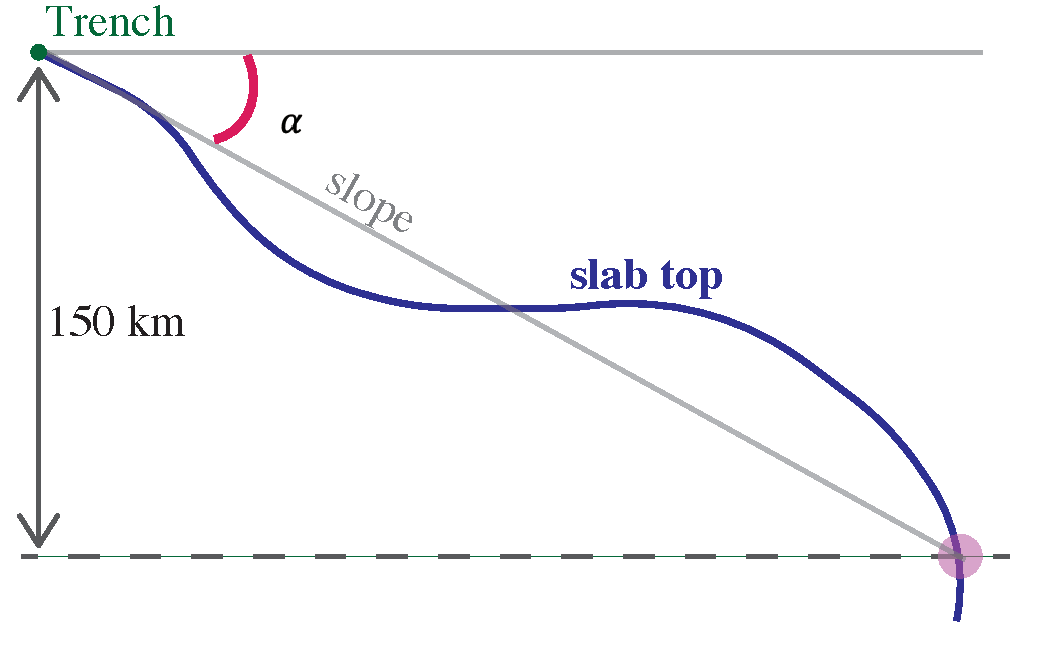
\includegraphics[width=4in]{dip_of_slab.pdf}
    \caption[本研究中隱沒傾角的計算方式]{本研究中隱沒傾角的計算方式。}
    \label{fig::dip_of_slab}
\end{figure*}

\begin{figure*}[ht!]
    \centering
    \includegraphics[width=4in]{Ref_Nazca_time_v2.pdf}
    \caption[智利參考模型隱沒板塊狀態隨時間變化]{智利參考模型隱沒板塊狀態隨時間變化。}
    \label{fig::Nazca_Ref_time}
\end{figure*}

模型中不同時間段的重力力矩與動水壓力力矩值如圖\ref{fig::Nazca_Ref_time}d所示。
本研究模型僅包含300公里以內的板塊段,因此在模型進行至8 Myr後,隱沒板塊長度並沒有顯著拉長,導致重力力矩量值恆定。
然而過去討論隱沒板塊幾何動力學的研究皆僅考慮410公里不連續面以上的作用力貢獻(\citealp{schellart2004quantifying}; \citealp{billen2008modeling}),因此本研究認為重力力矩在模型設定下的誤差不足以造成討論失真。

動水壓力力矩在模型進行10 Myr後開始急速增加,配合圖\ref{fig::Nazca_Ref_51}d與圖\ref{fig::Nazca_Ref_76}d模型動水壓力剖面,與隱沒板塊上、狹窄的地函楔低黏滯度通道處所產生的低壓帶有關,配合強烈彎曲的隱沒板塊下方高壓帶,導致隱沒板塊上下壓力差極大,造成隱沒系統中吸力增加。

\newpage
\section{墨西哥參考模型}
\subsection{初始模型設定}
墨西哥參考模型尺寸與智利參考模型相同,皆為長1200公里、深300公里的長方形二維剖面(見圖\ref{fig::reference Cocos model}),包含一段長760公里的海洋岩石圈與440公里的大陸岩石圈。
在海洋岩石圈絕對座標650公里處建立一段長70公里傾角60度的隱沒板塊。
\begin{figure*}[ht!]
    \centering
    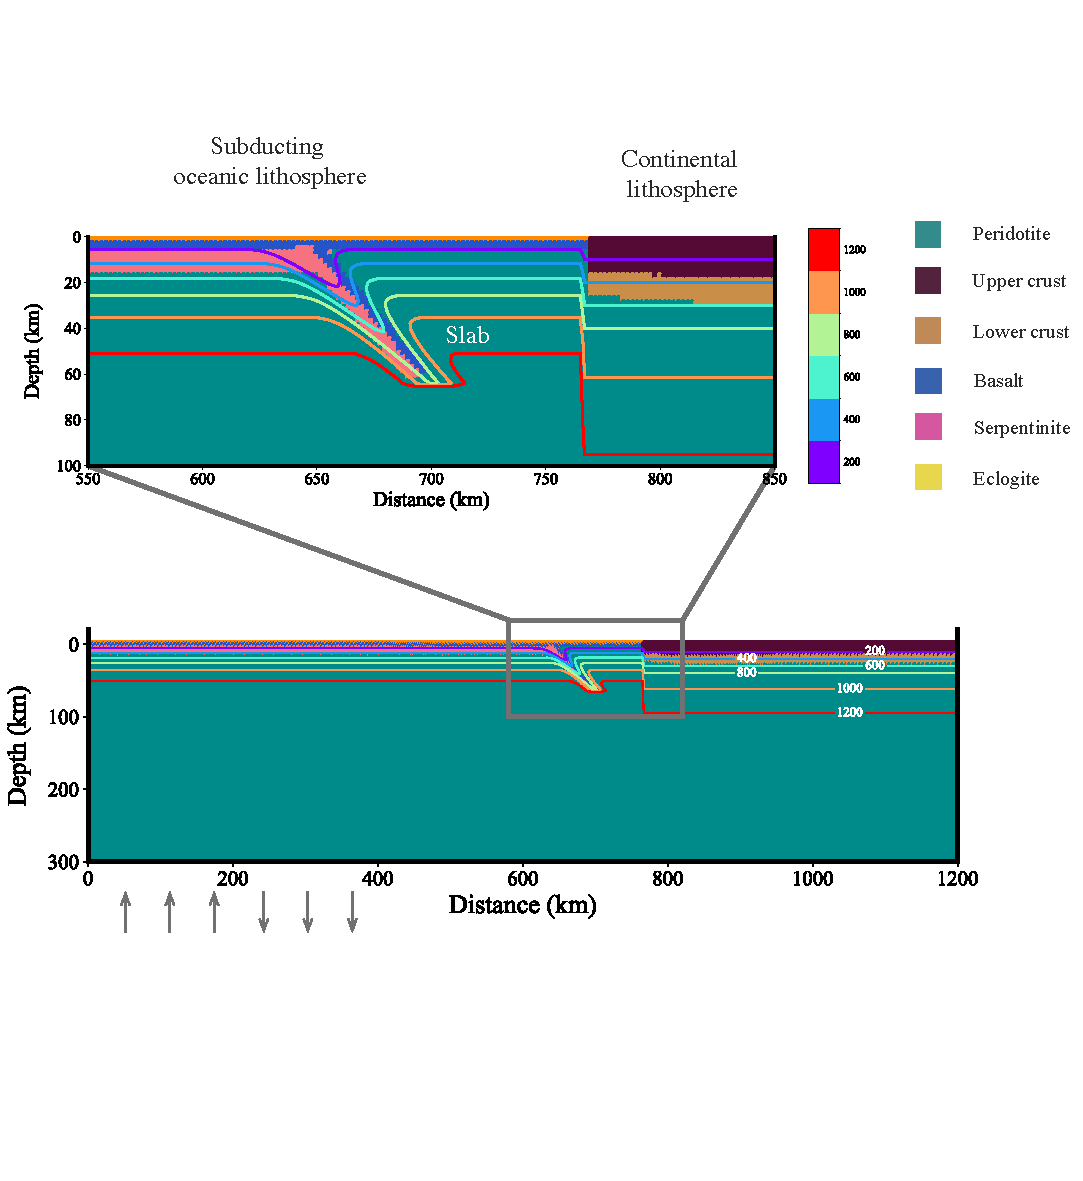
\includegraphics[width=6in]{Ref_Cocos.pdf}
    \caption[墨西哥參考模型設計與邊界條件示意圖]{墨西哥參考模型設計與邊界條件示意圖}
    \label{fig::reference Cocos model}
\end{figure*}

海洋岩石圈年齡為15個百萬年(\citealp{Manea2011Thermal}; \citealp{muller2019}),極為年輕,包含2公里厚的沉積物與6公里厚的玄武岩。由於從地球物理觀測資料得知科克斯板塊隱沒帶富含有大量水份,因此初始模型預設有10公里厚的綠泥岩,並且在隱沒過程中會產生10公里厚的蛇紋岩化橄欖岩。
海洋岩石圈熱構造由第二章式\ref{eq:Half Space Model}提及的半空間冷卻模型決定。
大陸岩石圈包含20公里厚的上部地殼與10公里厚的下部地殼,過去有不少研究討論墨西哥區域的熱構造,包含穩態模擬、地磁逆推獲得居禮溫度面與熱流資料研究。
本研究主要參考\citealp{Manea2011Curie}所模擬出的岩石圈熱構造,他們結合地磁逆推與隱沒帶模型模擬,推斷在40公里以上地殼地溫梯度每公里攝氏20$^{\circ}$,40公里以下地溫梯度每公里6度,至岩石圈底部為攝氏1330$^{\circ}$。
模型頂部邊界溫度為攝氏10$^{\circ}$,底部邊界溫度為攝氏1330$^{\circ}$。
模型左邊界以每年7公分速率往右移動,右邊界則固定不動。
本研究參考的速度同樣來自於\citealp{o2005uncertainties},與智利參考模型相同,模型上邊界為自由表面,而下邊界則為開放邊界,物質可自由進出。

本參考模型的岩石物理特性與智利參考模型類似,除了地函橄欖岩之外有較低的活化能之外,其餘物理性直接相同。
地函橄欖岩活化能的減少造成岩石強度比原先降低8$\%$。


\subsection{模型結果}\label{墨西哥參考模型結果}
墨西哥參考模型產生一深度約35-40公里、長度約80-100公里的平坦段。

在隱沒初始時期,由於海洋岩石圈極為年輕,此時海洋岩石圈等深度下溫度遠高於大陸岩石圈,因此模型早期玄武岩相變位置不斷往地函深處移動,於模型5 Myr時來到接近100公里深,如圖\ref{fig::Ref Cocos 26}a。
儘管如此,大陸岩石圈厚度約為100公里,相比於普通大陸岩石圈厚度較薄、溫度較高。
地函楔中橄欖岩融點因大量自由水加入而降低,在距離海溝100公里處發生部分熔融,如圖\ref{fig::Ref Cocos 26}c中黃色線段處。
同時劇烈的脫水作用導致大量蛇紋岩化橄欖岩在地函楔形成大範圍的低黏滯度區,如圖\ref{fig::Ref Cocos 26}b,促使地函流流動,增加地函楔溫度。
在近地表,海洋地殼上的沉積物、因變形而破碎的海洋地殼與蛇紋岩化橄欖岩在弧前區域堆積。
此時隱沒板塊以一相對高角度的狀態隱沒,角度可達50度,與正常的隱沒帶無異,隱沒角度隨時間變化如圖\ref{fig::Cocos Ref time}c。

在模型進行約略8 Myr時,隱沒板塊在深度30公里左右觸碰大陸岩石圈,隨後隱沒板塊角度開始快速下降,與動水壓力力矩顯著上升的時間點不謀而合,如圖\ref{fig::Cocos Ref time}d。
從圖\ref{fig::Ref Cocos 51}d模型動態壓力可見於地函楔頂部出現一低壓區,其與隱沒板塊下方因板塊彎曲所形成的高壓帶造成明顯的壓力梯度,因此造成動水壓力力矩增加。
同時間圖\ref{fig::Ref Cocos 51}c顯示在地函楔較深處持續發生部分熔融,在地表絕對座標700公里處有火山島弧生成。

隨後從10-15 Myr隱沒傾角逐漸降低,至接近15 Myr時模型達到平坦隱沒條件。
此時,地表上增積岩體累積厚大的沉積物,其所形成的弧前隆起高過火山島弧。
在隱沒板塊上方
這段時間隱沒板塊狀態直接影響岩漿作用特徵。
部分熔融比例幾乎呈指數減少,熔融量在平坦隱沒發育後趨近於0,暗示著火山活動停止,可見圖\ref{fig::Cocos Ref melting time}。
此外,部分熔融發生位置在5百萬年間往內陸移動超過50公里,暗示著地函楔攝氏60$^{\circ}$等溫線逐漸往內陸移動。

隨著隱沒持續進行,穩定的平坦隱沒於20 Myr後不再有明顯幾何上的改變,平坦深度維持在莫荷面之下,符合墨西哥區域的接收函數結果(\citealp{PerezCampos2008}),見圖\ref{fig::Ref Cocos 101}a、圖\ref{fig::Ref Cocos 126}a與圖\ref{fig::Ref Cocos 150}a。
隱沒地殼與大陸地殼交界處有一厚度約5公里的沉積物厚層,中間夾雜些許蛇紋岩化橄欖岩,這暗示著隱沒板塊平坦段雖然有長達100公里與大陸地殼接觸,然而交界處物質強度極弱,黏滯度低,很可能無法累積大量應力。
\citealp{Song2009}、\citealp{Song2012SC}利用地震學研究,皆有觀測得平坦段上的交界層為低速層。
\citealp{Song2012SC}更藉由非均相性認為其為經歷強烈剪切的變質岩成分。
\citealp{Manea2017}則認為該弱耦合物質為殘餘的蛇紋岩化橄欖岩。
在本參考模型中,獲得的低強度層應為沉積物主導、具有少部分蛇紋岩化橄欖岩的岩石成分。

值得一提的是,模型時間30 Myr的壓力剖面\ref{fig::Ref Cocos 150}顯示在大陸岩石圈進地表雖然有火山島弧,然而並沒有顯著的高壓區域,為另一弱偶和特徵的展現。
反觀於智利參考模型中壓力剖面自平坦隱沒發育後(\ref{fig::Nazca_Ref_76}d至\ref{fig::Nazca_Ref_126}d)便在上覆地殼近地表出現長達150公里的高壓區,顯示平坦隱沒於智利參考模型扮演著強耦合的角色。

\begin{figure*}[htp]
    \centering
    \includegraphics[width=6in]{Cocos_a0646frame_26_snapshot_5field_150_v1.pdf}
    \caption[墨西哥參考模型於5 Myr時之結果]{墨西哥參考模型於5 Myr時之結果。}
    \label{fig::Ref Cocos 26}
\end{figure*}

\begin{figure*}[htp]
    \centering
    \includegraphics[width=6in]{Cocos_a0646frame_51_snapshot_5field_150_v1.pdf}
    \caption[墨西哥參考模型於10 Myr時之結果]{墨西哥參考模型於10 Myr時之結果。}
    \label{fig::Ref Cocos 51}
\end{figure*}

\begin{figure*}[htp]
    \centering
    \includegraphics[width=6in]{Cocos_a0646frame_76_snapshot_5field_150_v1.pdf}
    \caption[墨西哥參考模型於15 Myr時之結果]{墨西哥參考模型於15 Myr時之結果。}
    \label{fig::Ref Cocos 76}
\end{figure*}

\begin{figure*}[htp]
    \centering
    \includegraphics[width=6in]{Cocos_a0646frame_101_snapshot_5field_150_v1.pdf}
    \caption[墨西哥參考模型於20 Myr時之結果]{墨西哥參考模型於20 Myr時之結果。}
    \label{fig::Ref Cocos 101}
\end{figure*}

\begin{figure*}[htp]
    \centering
    \includegraphics[width=6in]{Cocos_a0646frame_126_snapshot_5field_150_v1.pdf}
    \caption[墨西哥參考模型於25 Myr時之結果]{墨西哥參考模型於25 Myr時之結果。}
    \label{fig::Ref Cocos 126}
\end{figure*}

\begin{figure*}[htp]
    \centering
    \includegraphics[width=6in]{Cocos_a0646frame_150_snapshot_5field_150_v1.pdf}
    \caption[墨西哥參考模型於30 Myr時之結果]{墨西哥參考模型於30 Myr時之結果。}
    \label{fig::Ref Cocos 150}
\end{figure*}

\newpage
\subsection{墨西哥參考模型脫水位置與岩漿作用}
模型中發生部分熔融與海溝之距離與部分熔融量隨時間變化分別如圖\ref{fig::Cocos Ref melting time}a、b所示。模型中共可分成三段岩漿活躍時期與一段岩漿靜止期。

第一段岩漿活躍期在0-8 Myr隱沒早期,此時熔融量不多,以地函楔中的橄欖岩為主,主要發生在距海溝100公里處,為標準的島弧岩漿特徵。
第二段岩漿活躍期出現在8-20 Myr,由於平坦隱沒在8 Myr開始發育,因此當隱沒板塊發生幾何形狀改變後,部分熔融位置開始往內陸移動,從8-15 Myr之間共移動百餘公里。
岩漿靜止期始於平坦隱沒順利成形的15 Myr,此時因隱沒板塊逐漸貼近大陸地殼下方,莫荷面下的地函楔範圍逐漸縮小,故儘管發生部分熔融的位置不變,但部分熔融比例逐漸下降,熔融量趨近於0,最終地函楔橄欖岩部分熔融比例於模型進行20 Myr時達到最小值。
\begin{figure*}[h]
    \centering
    \includegraphics[width=5in]{Cocos_melting_time_series_v2.pdf}
    \caption[墨西哥參考模型岩漿作用隨時間變化]{墨西哥參考模型岩漿作用隨時間變化,灰色底標出平坦隱沒發育後時間段。(a)部分熔融與海溝之距離隨時間變化圖,縱軸中每個點代表每次部分熔融發生位置,顏色為指數上的部分熔融比例。(b)岩石熔融量隨時間變化圖,熔融量單位為每單位海溝產生之立方公里量中每20萬年瞬時量。顏色代表不同岩相。}
    \label{fig::Cocos Ref melting time}
\end{figure*}

隨後模型進入第三段岩漿活躍期,在20 Myr前,部分熔融狀態有一不連續間隔,熔融位置改變且熔融比例些微上升,如圖\ref{fig::Cocos Ref melting time}a,這暗示著岩漿作用源頭改變。
在該不連續時間段段後,部分熔融又重新以緩慢的速率往內陸遷移,與平坦隱沒平坦段的持續發育增長有關,隱沒板塊平坦段長度隨時間變化見圖\ref{fig::Cocos Ref time}a。
平坦隱沒具有與正常隱沒帶不同的溫壓路徑,由於其地殼在等深度下維持不變長達近80公里,在整段平坦段中壓力不變,但越靠內陸側之岩石溫度越高,此時鐵鎂岩相與沉積岩相很有可能會通過固熔點,導致海洋地殼發生部分熔融(\citealp{Gutscher2000Bcan})。
圖\ref{fig::Cocos Ref melting time}所統計之熔融岩相量顯示在20 Myr後陸續發生沉積物部分熔融,在23 Myr後橄欖岩熔融消失,此特徵與該地區的岩漿觀測研究相符(\citealp{ferrari2012dynamic})。
模型中岩漿活動將在第四章進行討論。

墨西哥參考模型的岩漿庫規模遠大於智利參考模型,累積的岩漿庫體積約是智利參考模型的100倍以上,根本原因為墨西哥參考模型的上覆板塊為高溫環境,而本研究所使用的岩漿庫冷卻參數與溫度高度相關,因此在墨西哥參考模型中,岩漿庫的冷卻速率緩慢,火山活動活躍。

將模型中部分熔融事件與岩漿庫絕對位置繪出,分別獲得圖\ref{fig::Cocos Ref 2Dtime series}a、b。
圖中顯示顯著的三段岩漿活躍期,第一段岩漿活躍期發生在絕對座標500至650公里、距海溝100公里之間,與正常的島弧岩漿活動特徵類似。
第二段岩漿活躍期發生在絕對座標650-750公里內,熔融深度、岩漿庫深度較第一段活躍期深,岩漿量也較大。
最終第三段岩漿活躍期發生在絕對座標750-830公里內,岩漿庫規模皆沒有前兩段活躍期大,但位置較集中,並且持續時間最長。

玄武岩至榴輝岩相變位置見圖\ref{fig::Cocos Ref 2Dtime series}c。
在模型早期,因隱沒岩石圈溫度比大陸岩石圈高,因此玄武岩至榴輝岩相變深度從40公里逐漸往接近100公里移動。
然而從圖\ref{fig::Ref Cocos 26}a與c可見儘管發生相變發生位置逐漸變深,該時期是一高角度隱沒帶,並沒有明顯的隱沒傾角趨緩特徵。
隨後在15 Myr之後,玄武岩相地殼來到模型時間段間最小長度,亦即玄武岩進入海溝後於15 Myr時會以最短的速度相變成榴輝岩相,圖\ref{fig::Cocos Ref time}d中顯示在15 Myr後重力力矩達到最高點,同樣可驗證該時間點為榴輝岩相長度達到模型中最大值,然而此時間剛好發生在平坦隱沒形成後不到一個百萬年。
因此,再次證明玄武岩相變與榴輝岩的出現仍然可以形成長久穩定的平坦隱沒。
隨後由於平坦隱沒地殼往內陸延伸的速度大於隱沒地殼增溫的速度,因此玄武岩相變深度再次往內陸推進。
平坦段中增溫速度緩慢顯示其上方沒有顯著的不可逆變形,因此摩擦熱不大,這進一步意味著平坦段上的應力狀態以低耦合為主,與觀測資料吻合(\citealp{moran2007cenozoic}, \citealp{PerezCampos2008})。

\begin{figure*}[ht]
    \centering
    \includegraphics[width=4in]{Ref_Cocos_2Dtime_series_v1.pdf}
    \caption[墨西哥參考模型部分熔融、岩漿庫與玄武岩相變時空關係圖]{墨西哥參考模型部分熔融、岩漿庫與玄武岩相變位置時空關係圖。(a)圓點為墨西哥參考模型不同時間的部分熔融發生位置,線條為每10 Myr的隱沒板塊頂部介面(分別為10 Myr, 20Myr, 30 Myr與40 Myr),橫軸上方標示出模型於40 Myr的相對海溝距離。(b)圓點為墨西哥參考模型不同時間的岩漿庫發生位置,線條為每10 Myr的隱沒板塊頂部介面(分別為10 Myr, 20Myr, 30 Myr與40 Myr),橫軸上方標示出模型於40 Myr的相對海溝距離。(c)圓點為墨西哥參考模型不同時間之玄武岩相變位置。}
    \label{fig::Cocos Ref 2Dtime series}
\end{figure*}

\newpage
\subsection{參考模型隱沒板塊與其轉動平衡}
模型中的平坦隱沒長度與深度隨時間變化見圖\ref{fig::Cocos Ref time}a, b,平坦段深度與長度的定義已於\ref{平坦隱沒定義}節提及。

在平坦隱沒發育初期,模型時間15-20 Myr之間平坦隱沒還在緩慢發育,並且玄武岩相變深度持續加深,因此儘管重力力矩逐漸下降,平坦段長度並沒有顯著增加,隨後於20 Myr後,重力力矩不再變化,平坦段開始增長,至30 Myr可到達超過100公里長。
儘管平坦隱沒段長度逐漸變長,然而模型中平坦隱沒段深度於全時段皆沒有劇烈改變,均落在30-40公里深上下。
平坦隱沒段長度與深度皆與觀測資料吻合。

模型中隱沒板塊於150公里之內的角度變化如圖\ref{fig::Cocos Ref time}c所示。
在模型早期,角度隨時間增加直到5 Myr,隨後隨著動水壓力力矩快速增加(圖\ref{fig::Cocos Ref time}d),隱沒傾角開使緩慢下降。
在模型時間15 Myr後,隱沒傾角不再劇烈改變,暗示平坦隱沒開始發育後,隱沒帶趨近穩定,不再有幾何形狀上的變化。

\begin{figure*}[hb]
    \centering
    \includegraphics[width=4in]{Ref_Cocos_time_v1.pdf}
    \caption[墨西哥參考模型隱沒板塊狀態隨時間變化]{墨西哥參考模型隱沒板塊狀態隨時間變化。紫色虛線為模型中平坦隱沒發育成形之開始時間。(a)模型中平坦段長度隨時間變化,其中}
    \label{fig::Cocos Ref time}
\end{figure*}

模型中不同時間段的重力力矩與動水壓力力矩值如圖\ref{fig::Cocos Ref time}d。
由於本參考模型有玄武岩相變位置改變的現象,因此重力力矩在時間軸上改變劇烈。
模型早期有顯著的玄武岩相變深度變化,然而在隱沒板塊觸碰到大陸地殼後,被動導致隱沒傾角逐漸減少,玄武岩相變深度逐漸回歸至50公里深,隱沒板塊溫度逐漸升高。
重力力矩在模型時間15 Myr達到最大值,隨後隨著平坦隱沒發育,玄武岩相變位置有水平方向上的變化,逐漸往內陸移動,導致重力力矩逐漸減小。

動水壓力力矩增加起始時間早於重力力矩,應發生於隱沒板塊觸碰到大陸地殼的瞬間開始大幅增加。
在平坦隱沒發育後,動水壓力力矩雖有上升趨勢,然而增加斜率緩慢。
導致本模型能維持平坦隱沒持續15 Myr的原因可能有兩種,
第一,因為玄武岩相變深度加深的現象導致重力力矩在15 Myr後持續減少,因此平坦隱沒能穩定存在。
第二,早在動水壓力力矩巨幅增加的時期,便已經決定整個隱沒系統的動態穩定。由於15 Myr後動水壓力力矩依然有極大的轉動力矩,因此無論重力力矩是否下降,平坦隱沒皆可穩定存在。